\section{Introduzione al Cloud Computing}
\subsection{Concetti preliminari}
\begin{definition}[Economia service-based]
L'economia si è spostata dal concentrarsi sui beni al concentrarsi sui servizi, e.g. comprarsi una bicicletta vs CicloPi (usufruire di un servizio) oppure in informatica i servizi di storage (Dropbox, Amazon S3)
\end{definition}

\subsubsection{QoS}
\begin{definition}[Quality of Service (QoS)]
fondamentale per qualsiasi servizio che utilizziamo, non basta che sia conveniente economicamente ma deve anche essere affidabile. Le informazioni sull’affidabilità vengono scritte nel \textit{Contratto} che i clienti spesso ignorano e accettano senza leggere.
\end{definition}

\subsubsection{SLA}
\begin{definition}[Service Level Agreement (SLA)]
Il SLA fa riferimento alla parte del contratto in cui viene stabilita l'\textbf{affidabilità del servizio}. Le percentuali fornite sono spesso forvianti, tipicamente si legge \textit{"99\% uptime"} ma è solo per ragioni di business e per stare al passo con i competitor del settore.
Il SLA è scritto da tre diverse figure: un avvocato, un business expert e un developer.
\end{definition}

\begin{figure}[h!]
    \centering
	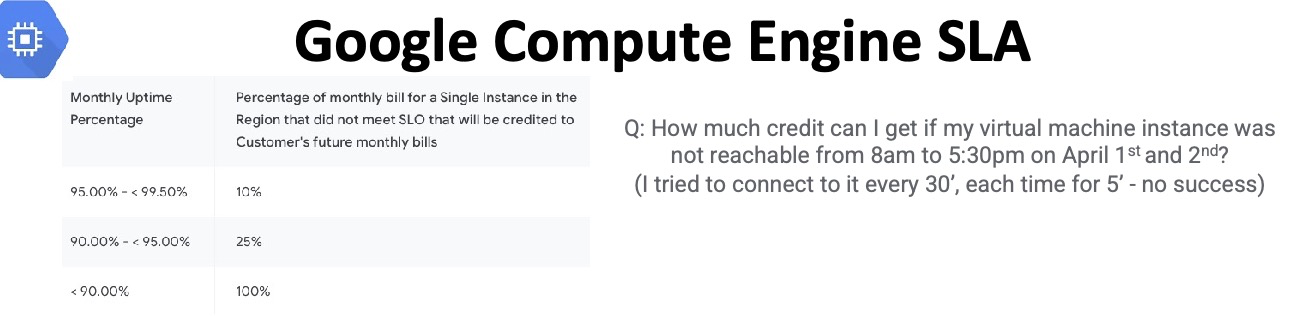
\includegraphics[width=0.7\textwidth]{1.png}
    \caption{Google rimborsa (sotto forma di credito) "fino al 100\%" delle spese in caso di downtime}
\end{figure}

\subsubsection{Uptime}
\begin{definition}[Monthly Uptime Percentage]
    $$\text{MPU = } \frac{\text{\# minuti in un mese - \# minuti di downtime}}{\text{\# minuti in un mese}}$$
\end{definition}

\newpage
\subsubsection{Downtime}
\begin{definition}[Downtime Period]
    \textbf{Minuti consecutivi} di downtime
\end{definition}
\paragraph{Come Google conteggia il downtime} I minuti parziali (e.g. 2m 30s) sono arrotondati per difetto (2m 30s $\rightarrow$ 2m), mentre qualsiasi downtime per un intervallo di tempo inferiore a 1 minuto non viene neanche considerato da Google.\\
Ma quindi quanto credito posso riavere indietro, nel caso in cui per due giorni di fila il servizio è down dalle 8 alle 17:30 e io provo a connettermi senza successo ogni 30 minuti, insistendo ogni volta per 5 minuti?\\
Risposta: il Monthly Uptime Percentage è $$ \text{MUP} = \frac{(30\cdot 24\cdot 60)-(2\cdot 20\cdot 5)}{30\cdot 24\cdot 60} = \frac{43000}{43200} = 0.955$$ quindi non rientro neanche nella soglia per il 10\%

\subsection{Errori comuni nell'adozione del Cloud}
\paragraph{Overprovisioning e Underprovisioning}
Quando si realizza un servizio è difficile predire quanto crescerà la domanda nel tempo e di conseguenza la quantità di risorse che saranno necessarie. In tal senso si parla di overprovisioning e underprovisioning.
\begin{definition}[Overprovisioning]
gestire in anticipo un eventuale flusso di utenti in crescita. Utilizzo overkill (eccessivo) di risorse rispetto a quelle effettivamente necessarie con conseguente spreco di risorse    
\end{definition}

\begin{definition}[Underprovisioning]
se il picco di utenti è sottostimato, il servizio risulterà in una cattiva user experience e gli utenti che non riescono ad accedere al servizio difficilmente ritorneranno
\end{definition}

\subsection{Vantaggi (alcuni) del Cloud}
Con il Cloud non serve fare previsione sulle richieste perché le risorse appaiono ”illimitate” agli occhi dell'utente e soprattutto disponibili on-demand. Il nome Cloud deriva dal fatto che quando si disegnava lo schema client-server, tutto ciò che stava fra i due veniva rappresentato come una nuvoletta per semplicità.\\
Dal punto di vista \textbf{economico}:
\begin{itemize}
    \item non servono un investimento e una progettazione iniziale per l’infrastruttura hardware, infatti si possono realizzare e offrire servizi hostati interamente sul Cloud
    \item servizi \textbf{pay-per-use}: paghi solamente ciò che usi, tipicamente vengono preferiti anche se si va a spendere di più perché garantiscono \textbf{elasticità} e permettono di \textbf{trasferire il rischio su terzi} cioè se qualcosa va storto il responsabile è il provider del servizio Cloud
    \item Il modello di business introdotto dal Cloud Computing permette di trasformare alcuni costi fissi in \textbf{costi variabili} e permette uno shift da spese CapEx a spese \textbf{OpEx}
\end{itemize}

\subsection{Modelli di servizio}
\paragraph{Infrastucture as a Service (IaaS)} fornisce server, memoria, rete (virtualizzati), il fornitore di servizi IaaS gestisce tutta l’infrastruttura. Il cliente è responsabile di tutti gli altri aspetti del deployment (per esempio sistema operativo, applicazione). Il mercato del Cloud IAAS è cresciuto del 31.3\% nel 2018. Esempi di IaaS sono \textbf{Amazon EC2} (instances) e \textbf{Amazon S3} (buckets)
\paragraph{Platform as a Service (PaaS)} fornisce un’intera piattaforma come un servizio (macchine virtuali, sistema operativo, servizi, ambiente di sviluppo), quindi il fornitore PaaS gestisce infrastruttura + sistema operativo + enabling software. Il cliente è responsabile di installare e gestire l’applicazione. Esempi di PaaS sono: Heroku, Azure, Google App Engine
\paragraph{Software as a Service (SaaS)} fornisce software on-demand accessibile mediante client thin o API, quindi il fornitore SaaS gestisce l’infrastruttura + sistema operativo + applicazione e il cliente non è responsabile di niente.  Esempi: Salesforce.com, Google Drive
La differenza tra IaaS e PaaS è lieve, se offri PaaS spesso sei obbligato a offrire anche IaaS

\newpage
\subsection{Modelli di deployment}
\paragraph{Pubblico}il vantaggio è la scalabilità, però l'utente ha poco controllo su come sono gestiti i dati (ad esempio se succede qualcosa nei datacenter di Amazon, i nostri dati sono violati)
\paragraph{Privato} non ha molta scalabilità però c'è più sicurezza di dati
\paragraph{Ibrido} soluzione molto utilizzata, si tengono sul cloud privato i dati sui quali si vuole avere pieno controllo e privacy, i restanti su un cloud pubblico fornito da un cloud provider

\begin{figure}[h!]
    \centering
    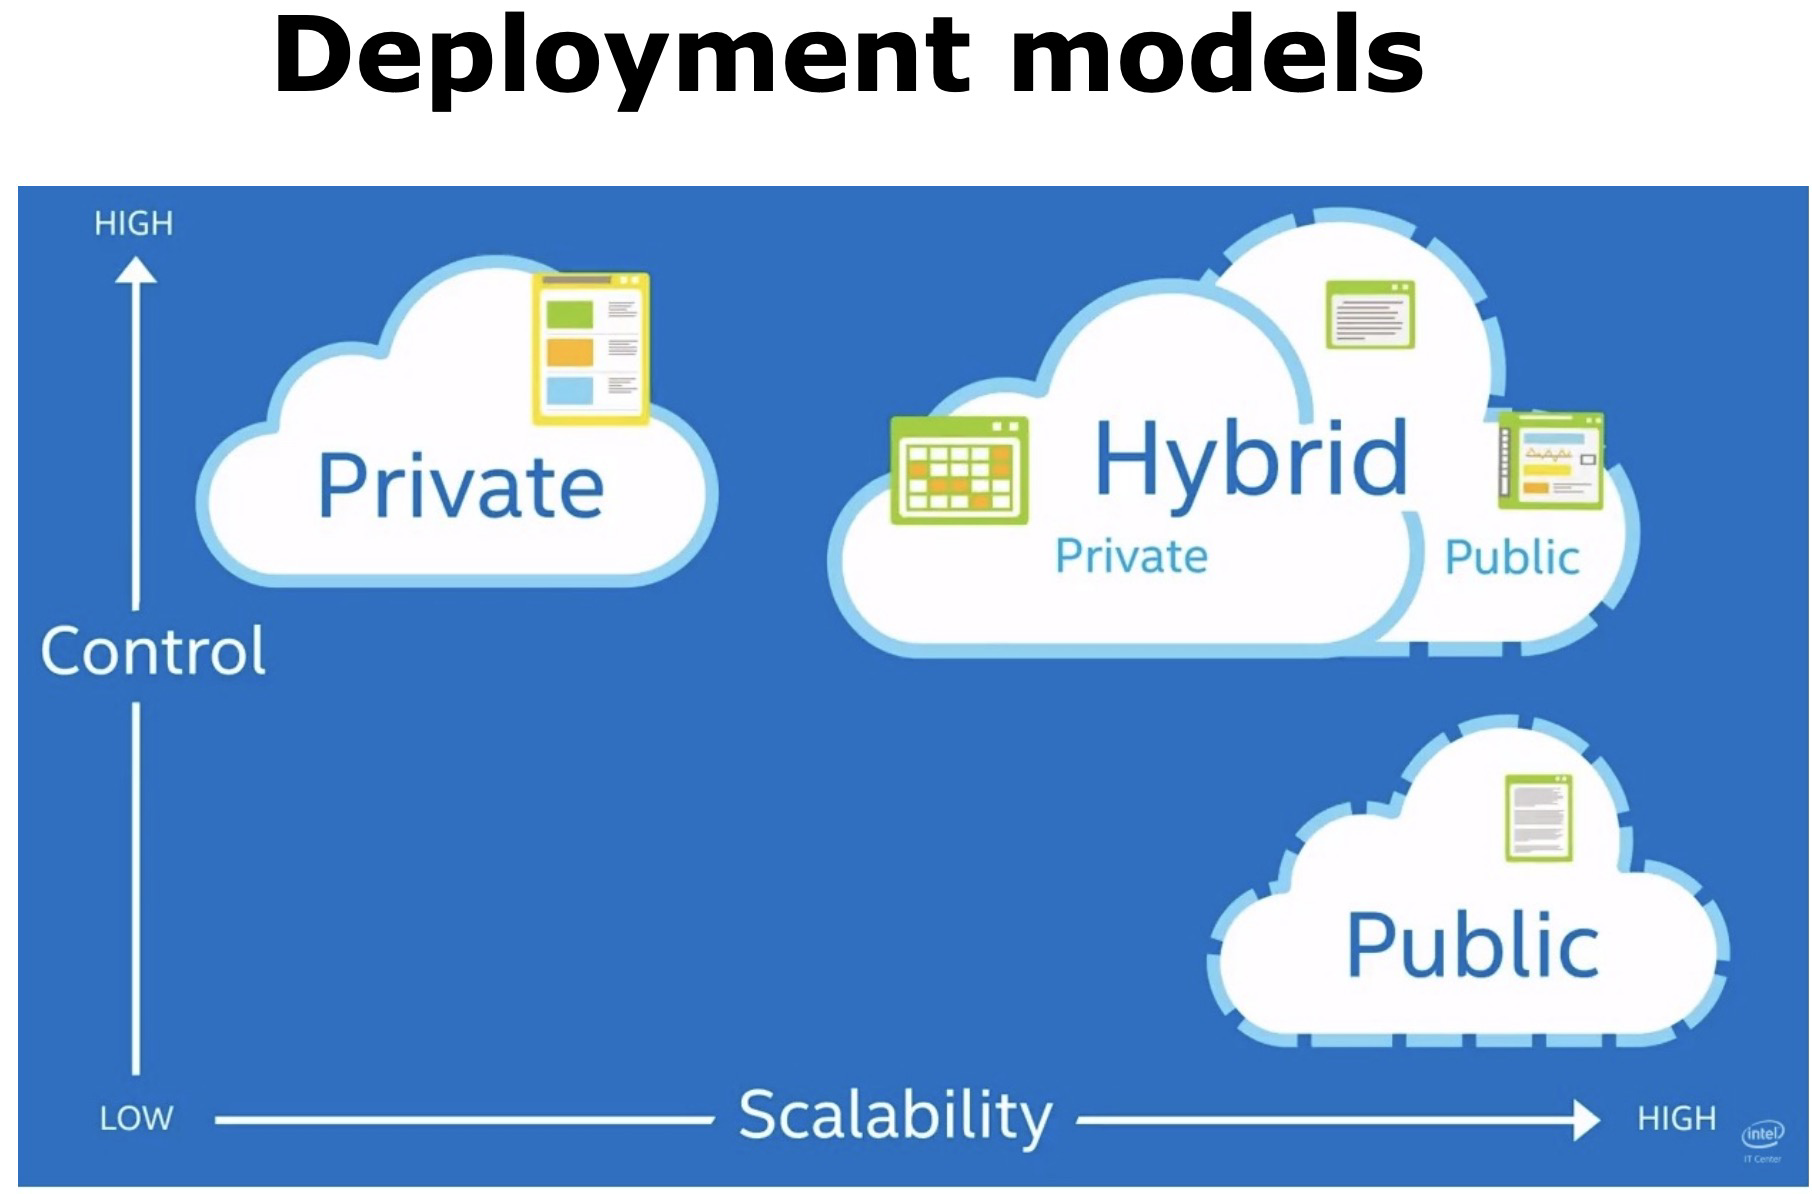
\includegraphics[width=0.7\textwidth]{2.png}
    \caption{trade-off da considerare per i vari tipi di deployment}
    %\label{fig:enter-label}
\end{figure}

\subsection{Ostacoli per l'adozione del Cloud}
\begin{itemize}
    \item \textbf{Confidenzialità dei dati}: dove verranno memorizzati i nostri dati concretamente? Privacy e integrità dei dati sono garantiti? Come? Come si può sapere se si è verificato un problema?
    \item \textbf{Disponibilità dei servizi}: cosa succede se un Cloud provider fallisce? Spesso le aziende si affidano ad un solo Cloud provider ma bisogna usarne di più (no \textit{single point of failure}, il sistema deve essere fault tolerant). Bisogna anche mettere in conto che ci saranno dei fallimenti temporanei e il servizio potrebbe non essere disponibile in alcuni momenti
    \item \textbf{Vendor lock-in}: più vengono utilizzate funzioni del Cloud più si rimane ”incatenati” all'ecosistema di quel provider perché se proviamo a spostare i nostri dati altrove dovremmo modificare tutte le nostre applicazioni per portarle su altri Cloud. Si tratta di un lock-in tecnologico legato alla difficoltà nella transizione verso un altro provider, non c'è nessuna clausola contrattuale che impedisce di abbandonare l'ecosistema del provider
\end{itemize}